% !TEX TS-program = pdflatex
% !TEX encoding = UTF-8 Unicode

% TeX-M (r1.1)
% For my math classes at UT Austin
% Notes template created by Abdon Morales for the College of Natural Science
% and for the Department of Mathematics and Computer Science
% (c) 2019 - 2024 Abdon Morales and the University of Texas at Austin
% This is a notes template for a LaTeX document using the "article" class for Mathematics (Calculus)
% at the University of Texas at Austin.

% Last change made: Jan 27, 2024 1:40 AM CST

% See "book", "report", "letter" for other types of document.

\documentclass[11pt]{article} % use larger type; default would be 10pt

% Start of Article customization options and addons (for more help and information reference to Overleaf's guides and docs on Latex.
\usepackage[utf8]{inputenc} % set input encoding (not needed with XeLaTeX)

%%% Examples of Article customizations
% These packages are optional, depending whether you want the features they provide.
% See the LaTeX Companion or other references for full information.

%%% PAGE DIMENSIONS
\usepackage{geometry} % to change the page dimensions
\geometry{letterpaper} % or letterpaper (US) or a5paper or....
% \geometry{margin=2in} % for example, change the margins to 2 inches all round
% \geometry{landscape} % set up the page for landscape
%   read geometry.pdf for detailed page layout information

\usepackage{graphicx} % support the \includegraphics command and options
\usepackage{xcolor}

% \usepackage[parfill]{parskip} % Activate to begin paragraphs with an empty line rather than an indent

%%% PACKAGES
\usepackage{booktabs} % for much better looking tables
\usepackage{array} % for better arrays (eg matrices) in maths
\usepackage{paralist} % very flexible & customisable lists (eg. enumerate/itemize, etc.)
\usepackage{verbatim} % adds environment for commenting out blocks of text & for better verbatim
\usepackage{subfig} % make it possible to include more than one captioned figure/table in a single float
\usepackage{exercise}
% Math tools
\usepackage{mathtools}
\usepackage{amsmath}
\usepackage{tikz} % For charts, mathematical graphs, and etc
%% Equal symbol for L'Hospital Rule
\usepackage{tcolorbox}
\newcommand\LR{\stackrel{\mathclap{\normalfont\mbox{L.R}}}{=}}
% These packages are all incorporated in the memoir class to one degree or another...

%%% HEADERS & FOOTERS
\usepackage{fancyhdr} % This should be set AFTER setting up the page geometry
\pagestyle{fancy} % options: empty , plain , fancy
\renewcommand{\headrulewidth}{0pt} % customise the layout...
\lhead{}\chead{}\rhead{}
\lfoot{}\cfoot{\thepage}\rfoot{}

%%% SECTION TITLE APPEARANCE
\usepackage{sectsty}
\allsectionsfont{\sffamily\mdseries\upshape} % (See the fntguide.pdf for font help)
% (This matches ConTeXt defaults)

%%% ToC (table of contents) APPEARANCE
\usepackage[nottoc,notlof,notlot]{tocbibind} % Put the bibliography in the ToC
\usepackage[titles,subfigure]{tocloft} % Alter the style of the Table of Contents
\renewcommand{\cftsecfont}{\rmfamily\mdseries\upshape}
\renewcommand{\cftsecpagefont}{\rmfamily\mdseries\upshape} % No bold!
%%% END Article customizations

%%% The "real" document content comes below...

\title{Recessions, Expansions, and the Debate over how to manage them}
\author{Abdon Morales \\ The University of Texas at Austin \\ ECO 304L \\ Wayne Geerling}
\date{\date \\ Week 8 : Chapter 14}
%\date{} % Activate to display a given date or no date (if empty),
         % otherwise the current date is printed 

\begin{document}
\maketitle
\subsection*{The Great Depression was unlike any recession we've experienced since.}
The Great Depression of the 1930s gave birth to macroeconomics as a subdiscipline of economics. Previously, economists generally focused on microeconomics: they emphasized the interaction of supply and demand in individual markets; but the depth and duration of the Great Depression forced economists to pay more attention to overall economic aggregates.

In the midst of the Depression, photographer Dorothea Lange documented the plight of migrant farm workers in California, thousands of whom were living in open-air camps and nearly starving. Driving north on Highway 101, Lange spotted Florence Owens, a mother tending to five of her children while her husband and the two oldest boys hiked into town to try to get the family's broken-down car fixed. Published in the \textit{San Francisco News}, Lange's photos of Owens and her children quickly became iconic images of Americans beaten down by the hardships of the time but determined to persevere.

Although according to official statistics, the economy had started to turn the corner, people like Owens and her family had several lean years ahead of them. The same was true elsewhere in the world, because the Great Depression was a sobering shock to the entire global economy, after the rapid industrial growth of the decade before.

Fortunately, we've not seen anything so severe since the Great Depression; however, recessions do still occur. In this chapter, we use our aggregate demand-aggregate supply (AD - AS) model to examine some causes of GDP stagnation and high unemployment. We also look closely at three major contractions in U.S history: the Great Depression of the 1930s, the Great Recession from 2007 to 2009, and the coronavirus-caused recession that began in 2020. We then consider some of the major debates about the macroeconomy; all of this sets us up for coverage of government policy responses to business cycles: fiscal policy (Chapter 15 and 16) and monetary policy (Chapter 17 and 18).

\begin{tcolorbox}[width=\textwidth,colback={white},title={Big Questions},colbacktitle=yellow,coltitle=blue]
\begin{itemize}
\item Why do recessions occur?
\begin{itemize}
\item Shifts in aggregate demand.
\item Shifts in aggregate supply.
\end{itemize}
\item What happened during three major recessions?
\begin{itemize}
\item The Great Recession was characterized by shifts in both long-run aggregate supply and aggregate demand.
\item The Great Recession was deeper and longer than typical U.S recessions.
\item The Great Depression was significantly worse than the Great Recession.
\item The coronavirus recession was driven primarily by significant negative supply shock that decreases short aggregate supply (SRAS). However, aggregate demand (AD) also declined.
\end{itemize}
\item What are the big disagreements in macroeconomics?
\begin{itemize}
\item The big debates in macroeconomics focus on the flexibility of prices and the emphasis on aggregate supply or aggregate demand. The two key schools of thought are classical economics and Keynesian economics.
\item If prices assumed to be flexible, the implication is a generally stable macroeconomy without significant need for government help.
\item If prices are assumed to be sticky, the implication is inherently unstable economy in need of government assistance.
\end{itemize}
\end{itemize}
\end{tcolorbox}

\section*{Why do recessions occur?}
Recessions are short-term economic downturns typically characterized by declines in real GDP growth and increases in the unemployment rate. We can use our AD-AS model to examine some different causes of recessions; in this section, we first consider a decline in aggregate demand and then turn to a decline in aggregate supply.

\subsection*{Declines in Aggregate Demand}
Aggregate demand changes in response to many different factors. In Chapter 13, we divided these into four groups: consumption factors, investment factors, government spending, and net export factors; when aggregate demand declines, the economy moves to a new equilibrium, with lower real GDP and higher unemployment. We illustrate a decline in AD in Figure 14.1. The economy is initially in long-run equilibrium at point A, with full-employment at \(Y\)*, unemployment at its natural rate \(u\)*, and the price level at 100. When aggregate demand declines from \(\text{AD}_0\) to \(\text{AD}_1\), the economy moves to a new, short-run equilibrium at point B.(Recall that long-run equilibria are denoted with upper-case letters, and short-run with lower-case.) The short-run equilibrium is characterized by lower real GDP and a higher unemployment rate - standard recession conditions.

\begin{center}
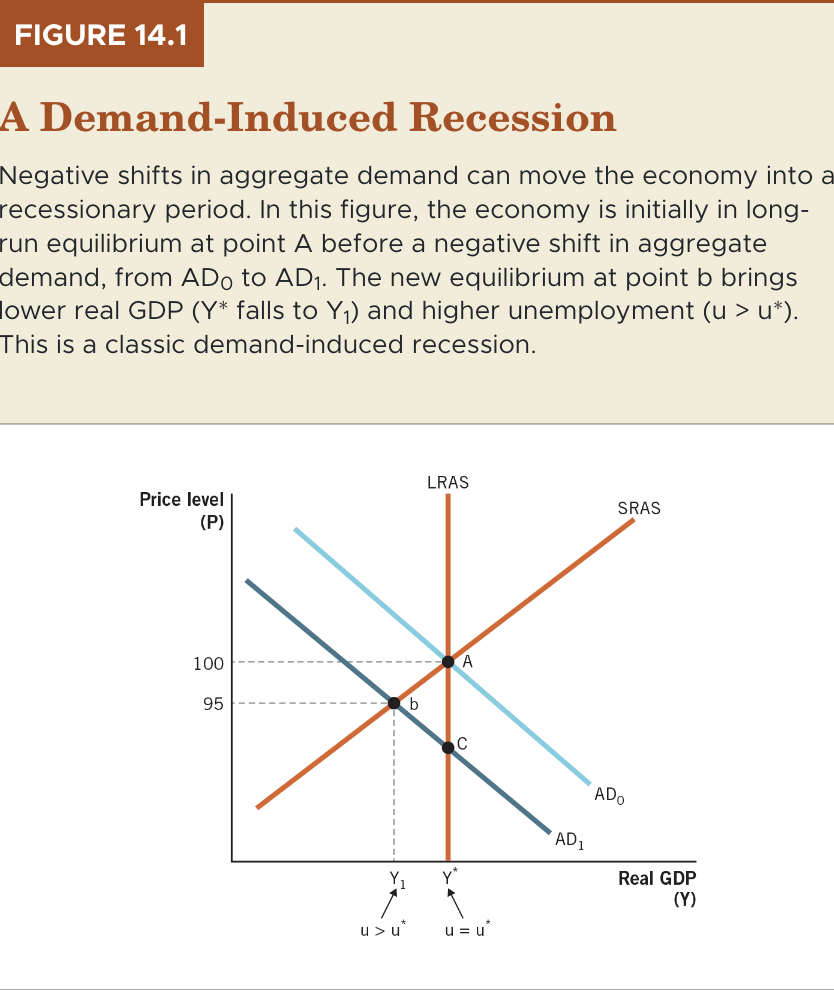
\includegraphics[scale=0.5]{images/Figure 14.1.png} 
\end{center}
As we have discussed in Chapter 13, if prices adjust downward in the long run, eventually the economy moves to a new long-run equilibrium at point C, with full-employment output (\(Y\)*) restored and unemployment back to the natural rate (\(u\)*); but the short run is painful. Laid-off workers suffer from lost income, and the retail locations and factories where they worked may be shuttered, no longer generating corporate tax revenue (and instead becoming targets for vandals). To minimize these effects, elected representatives and policymakers often look for ways to help move the economy back to full employment by shifting aggregate demand back to its initial level (\(\text{AD}_0\)). Economists generally feel that periods of high unemployment are the times when demand-stimulating governmental policies are most effective. Policy options include government spending increases, tax cuts, and expansionary monetary policy. (These are each discussed in the next four chapters.)

Many, if not all, recessions can be characterized by a fall in aggregate demand. Even when a decline in aggregate demand is not the initial cause, it often compounds problem, as people spend less due to drops in consumer or business firm confidence.

\subsection*{Declines in aggregate supply}
Recession conditions, with high unemployment and lower real GDP, can also be caused by declines in aggregate supply, either short run or long run. First, consider short-run decline; recall that this happens when input prices rise...because oil and gasoline are important inputs for many production processes, these price jumps constituted a supply shock that caused the short-run aggregate supply curve to shift back. This is illustrated in Figure 14.2. Initially, the economy is in long-run equilibrium at point A, at full-employment output (\(Y\)*), and with the natural rate of unemployment (\(u\)*); but the supply shock (the oil and gas price increases) shifts short-run aggregate supply from \(\text{SRAS}_0\) to \(\text{SRAS}_1\). This shift moves the economy to a new short-run equilibrium (at point b) characterized by lower real GDP and higher unemployment. If the oil price spike is temporary, short-run aggregate supply eventually returns to its initial level (\(\text{SRAS}_0\)), and the economy returns to long-run equilibrium at A.

\begin{center}
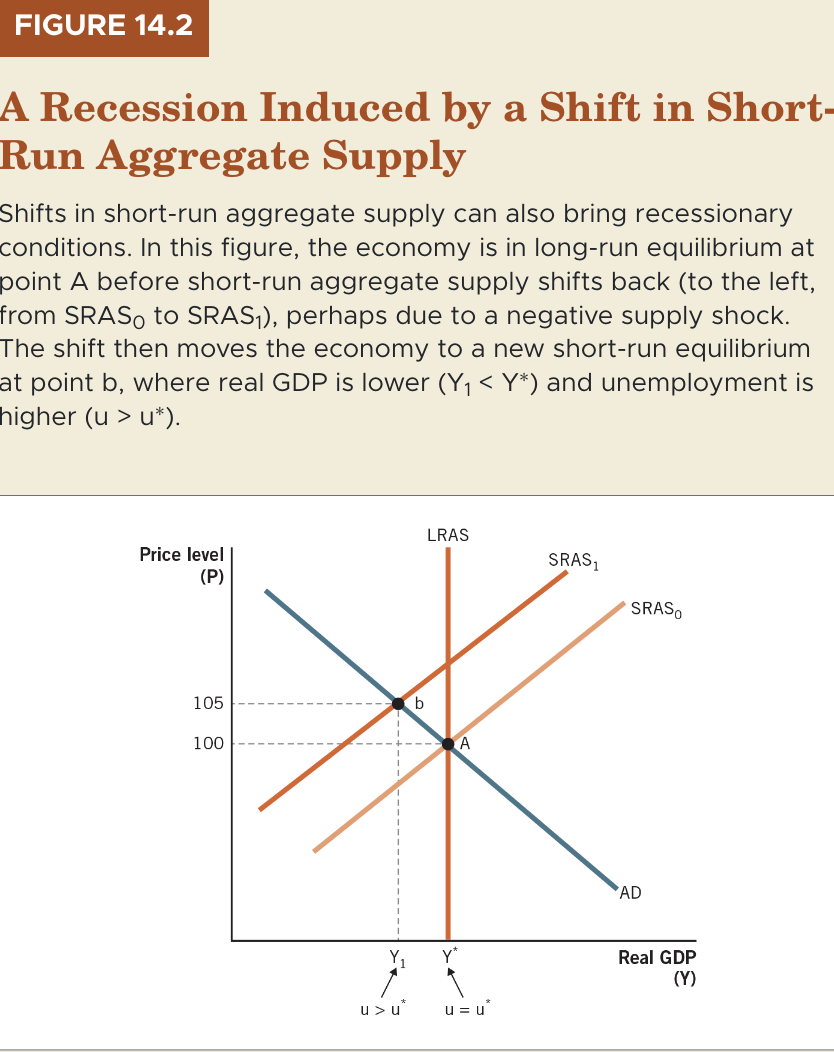
\includegraphics[scale=0.5]{images/Figure 14.2.png}
\end{center}
Now let's consider a decline in long-run aggregate supply; this is caused by negative changes in resources, technology, and institutions. An extreme example is a war fought on home soil; it destroys both labor and capital resources, as soldiers die and buildings or other tools are ruined, but whatever the cause is war, natural disaster, or something else, a reduction in resources means full-employment output declines and the long-run aggregate supply curve shifts to the left. This is illustrated in Figure 14.3; the reduction of resources moves the economy from long-run equilibrium at point A to a new long-run equilibrium at point B, assuming no other changes take place in the economy. At the new equilibrium, the economy is at a new full-employment level of GDP (\(Y\)**), while the unemployment rate is technically at the new natural rate of \(u\)**, this rate is often higher than the old unemployment rate, since jobs are shifting around in the economy, and this leads to more structural and frictional unemployment. While it's fortunately rare, this type of downturn is particularly painful, because there may not be a policy fix to move the economy back to its initial output level. All new economic growth takes place from the new baseline of (\(Y\)*).

As we move on, remember that no two recessions are exactly alike; we've just considered shifts in aggregate demand, short-run aggregate supply, and long-run aggregate supply. In the context and on the chalkboard, it is easy to shift curves and see immediate results. In real life, it is not always clear what is happening, especially during an actual recession. In the next section, we consider the three worst recessions in the past century.

\begin{center}
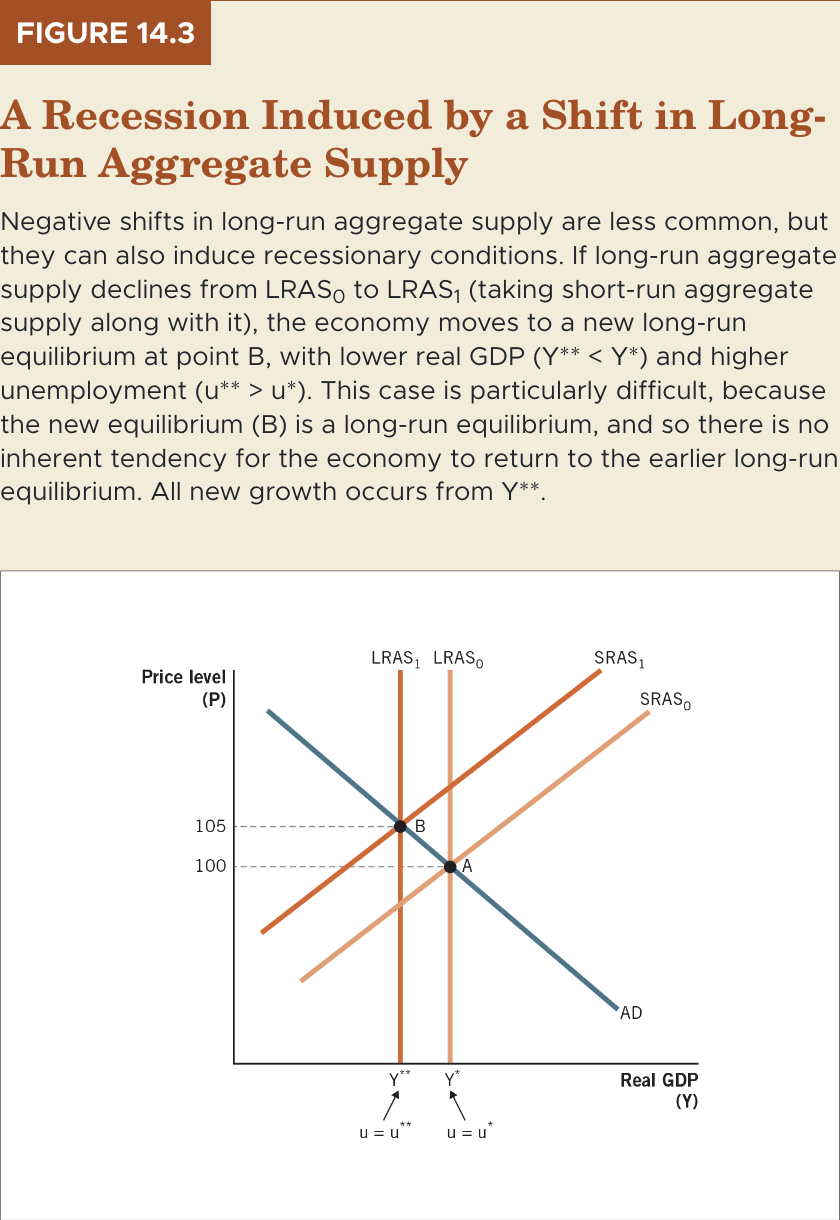
\includegraphics[scale=0.5]{images/Figure 14.3.png}
\end{center}

\section*{What happened during three major recessions?}
In this section, we look at three major economic contractions in U.S history: the Great Depression of the 1930s, the Great Recession (2007-2009), and the coronavirus recession of 2020. With each one, we begin with historical perspective and then move to analysis within our aggregate demand-aggregate supply model. This demonstrates the helpfulness of the model and prepares us to think about future recessions.

\subsection*{The Great Depression}
Going into 1929, the United States was full of optimism; World War I was a distant memory, the country's industrial sector was expanding - it was the "Roaring Twenties." All of that changed with the Great Depression, the single biggest economic contraction in the United States has experienced.
\subsubsection*{The Magnitude of the Great Depression}
To convey the historic magnitude of the Great Depression, Figure 14.4 plots U.S real GDP all the way from 1870 to 2019. We can quickly pick out the single worst economic incident over that long haul - it's the massive drop around 1930. There have been other contractions in the U.S economy since 1870, but none even come close to the Great Depression in severity. Real GDP fell from \$1,253 billion in 1929 to \$923 billion in 1933 (both in 2020 dollars); imagine a recession so sever that four years later the economy is producing 30\% less.

\begin{center}
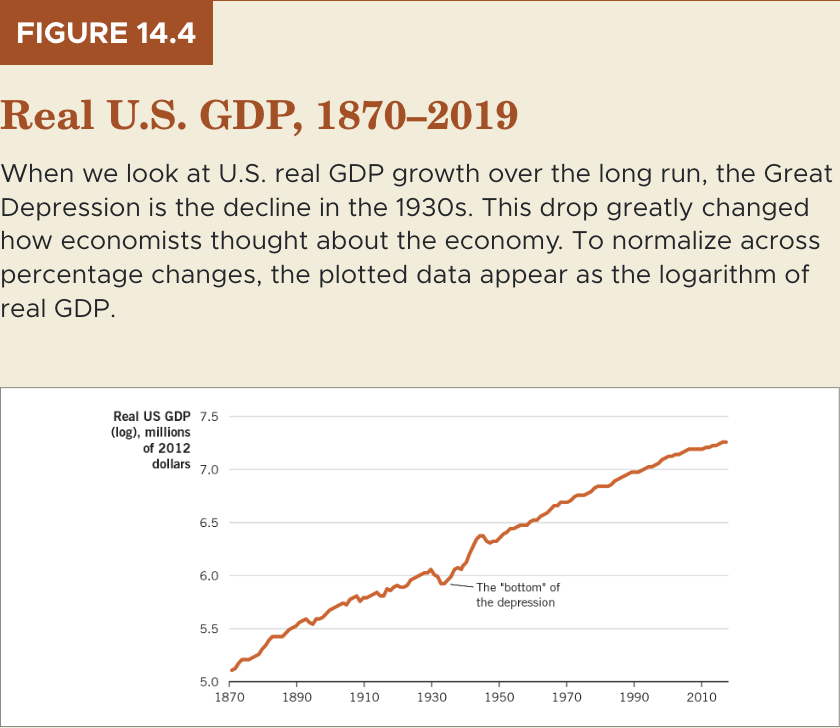
\includegraphics[scale=0.5]{images/Figure 14.4.png}
\end{center}
Panel (a) of Figure 14.5 moves in for a closer look, showing real GDP during the Depression years, 1929 to 1944. Real GDP fell by nearly a third from 1929 to 1933, and then took another three years just to recover to its pre-recession level. Panel (b) plots the unemployment rate over the same time frame; in 1930, the unemployment level was only 2.2\%, but just three years later it had climbed to over 25\%! In other words, by 1933 one in four workers was without a job. Particularly alarming was the length of the Depression: the unemployment rate remained above 15\% for almost the entire decade of the 1930s. In the 90 years since the Great Depression ended, the U.S unemployment rate has never again topped 15%.
\subsubsection*{Using our model to explain the Great Depression}
The Great Depression was actually two separate recessions: August 1929 to March 1933 and May 1937 to June 1938; (There's no technical distinction between a recession and a depression - the latter is really just a severe recession.) but here's something striking: even though real GDP finished the 1930s higher than it started, prices declined over the same period. At the end of the 1930s, the price level (measured by the GDP deflator) was still 20\% lower than in 1929; the decline in prices tells us that the primary cause of the Great Depression was a drop in aggregate demand.

\begin{center}
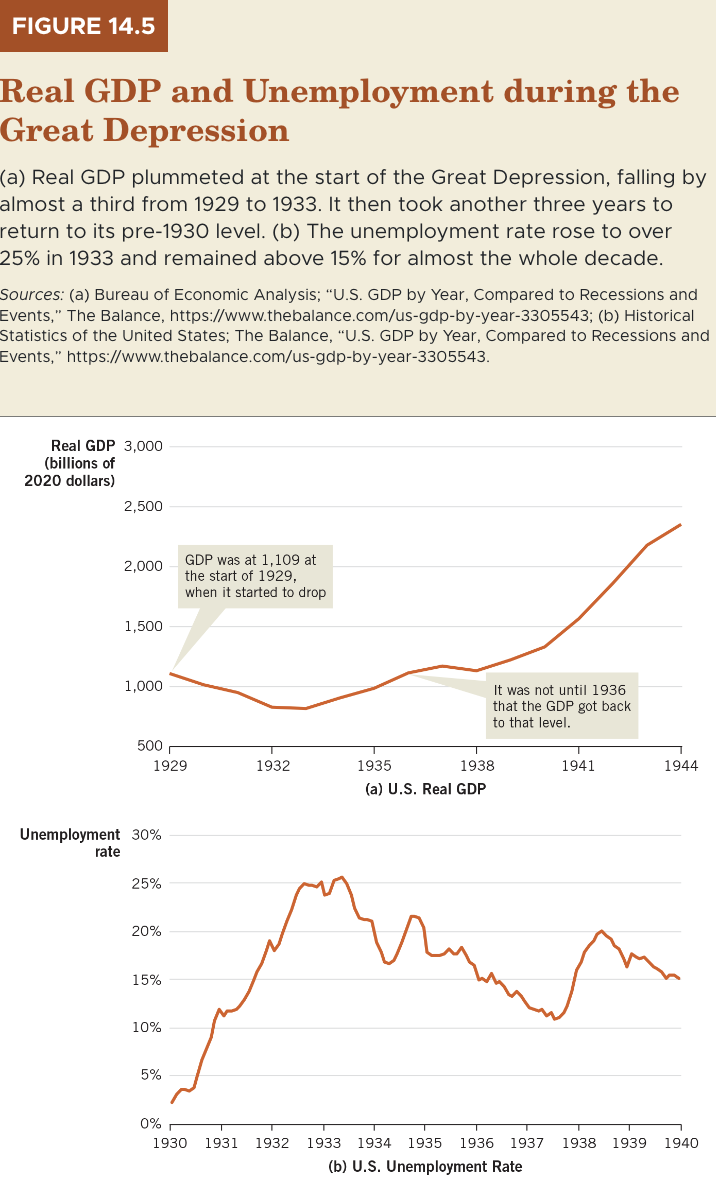
\includegraphics[scale=0.5]{images/Figure 14.5.png} 
\end{center}
Figure 14.6 illustrates what happened; in 1929, the economy was in equilibrium at point A, with aggregate demand \(\text{AD}_{1929}\). The a significant decline in aggregate demand took place over several years, as indicated by a shift to \(\text{AD}_{1930+}\); as we have seen, lower aggregate demand leads to lower real GDP (shown in the figure as \(Y_1\), higher unemployment rates (25\%), and a lower price level (shown here as a decline from 100 to 80). These outcomes match the symptoms of the Great Depression.

There were multiple causes of this aggregate demand decline; first, there was a decline in real wealth. The stock market crashed, beginning on October 24, 1929 (now known as "Black Thursday"); between 1929 and 1932, stock prices (as measured by the Dow Jones Industrial Average) fell by almost 90\%, but the Depression wasn't caused by the stock market crash alone. A second factor was a significant change in people's expectations, in reaction to the crash; in particular, expected future income declined-and we know that this factor decreases aggregate demand. When people expect to earn less in the future, they start spending less in the present.

\begin{center}
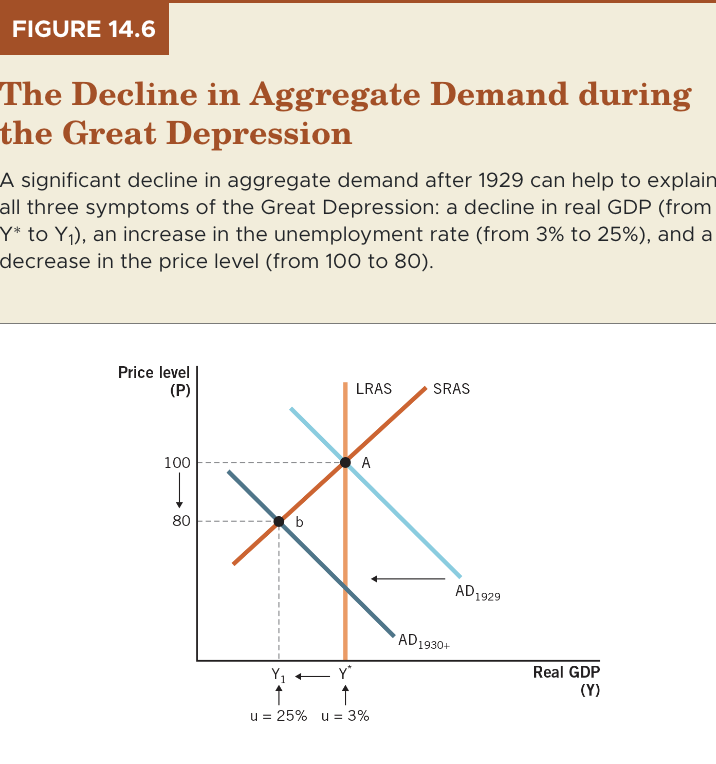
\includegraphics[scale=0.5]{images/Figure 14.6.png} 
\end{center}
The third and final cause, however, was the most important; unfortunately, it turns out that much of the decline in aggregate demand was due to misguided macroeconomic policy; \textbf{\underline{Macroeconomic policy}} encompasses governmental acts that influence the direction of the overall economy. Economists distinguish two different types of macroeconomic policy: fiscal policy and monetary policy. \textbf{\underline{Fiscal policy}} comprises the use of the government budget tools - government spending and taxes - to influence the macroeconomy; \textbf{\underline{Monetary policy}} involves adjusting the money supply to influence the economy. We're not yet ready to talk in detail about macroeconomic policies (those are the topics of the next section of this book), but we can consider the policy blunders in the context of our aggregate demand - aggregate supply model.

First, consider monetary policy; the government actually reduced the quantity of money in the economy in 1928 and 1929, in hopes of controlling stock prices that policymakers thought were too high. We know that reductions in the money supply lead to lower aggregate demand; then, when financial panic spread, many people withdrew deposits from their banks. As a result, more than 9,000 banks failed in the United States between 1929 and 1933; and while the government had the ability to lend to these ailing banks, it failed to do so. This led to even more shrinking of the money supply; in fact, between 1929 and 1933, the quantity of money circulating through the U.S economy declined by a third. Economists today agree that these policy failures led to a significant decline in aggregate demand and were a significant contributor to the economic contraction in the beginning years of the Great Depression.

There were other reasons why the Great Depression dragged on for so long; in the early 1930s, Presidents Hoover and Roosevelt raised taxes to try to balance the federal budget, but higher taxes also reduce aggregate demand. Another policy blunder affected aggregate supply: in 1930, Congress passed the Smoot - Hawley Tariff Act. This legislation imposed tariffs (taxes) on thousands of imported goods and set off a global trade war as other nations reacted by imposing tariffs on U.S exports.

In the end, most analysts agree: the Depression is best characterized by a significant decline in aggregate demand. In the section, we consider a modern recession with many similarities to the Great Depression. This recession occurred during your lifetime.

\subsection*{The Great Recession}
In December 2007, the United States entered the Great Recession; the name, which reflects the length and depth of the downturn compared to typical recessions, also reminds us that some of the causes resemble those of the Great Depression (like significant problems in the financial markets). The title stuck when the effects of the recession refused to subside for several years after the recession was officially over.

\subsubsection*{The Depth and duration of the Great Recession}
Officially, the Great Recession lasted 18 months, until June 2009, making it the longest of all recessions since World War II. Even so, this statistic understates how severely the U.S economy was affected; for several years after the recession was technically over, unemployment remained high and real GDP grew slowly. Figure 14.7 shows U.S real GDP in panel (a) and the unemployment rate in panel (b), both for the years 2005 to 2015; notice how real GDP didn't return to its pre-recession level for almost four years. During a typical recession, real GDP falls slightly and then bounces back after about a year and a half. Even worse, the unemployment rate took nearly seven years to drop back below 6\%.

Why was the Great Recession so severe? We'll use our aggregate demand and aggregate supply model to answer this question.
\subsubsection*{Using our model to explain the Great Recession}
At first, most economists and policymakers assumed that the Great Recession was caused exclusively by lower aggregate demand; but while aggregate demand did indeed fall, hindsight reveals issues with aggregate supply, too.

Two main factors contributed to a large decrease in aggregate demand; the first was a fall in real wealth, due to a severe drop in housing prices beginning in 2007. Figure 14.8 shows home prices from 2000 to 2020; notice the drop that began in 2007 and continued until 2011. People's homes are often the largest component of their wealth, so when real estate values fall, people's wealth drops; on top of that, U.S stock shares lost a third of their value during 2008. For millions of people, this meant a massive loss of retirement savings; both events contributed to large declines in real wealth, leading to lower aggregate demand.

\begin{center}
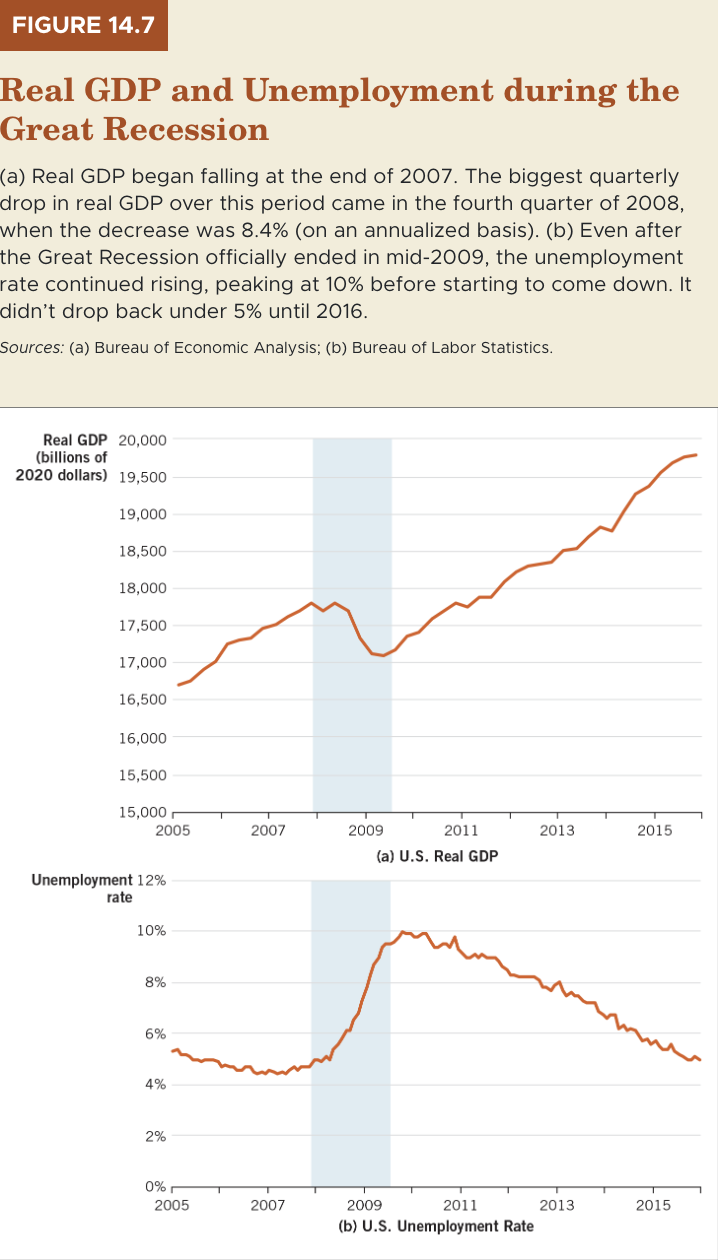
\includegraphics[scale=0.4]{images/Figure 14.7.png} 
\end{center}
The second big reason why aggregate demand fell was a decline in expected future income; beginning in 2007, consumers realized that the economy was slowing down. Their expectations of future income went down; a popular measure of consumer confidence, the Consumer Sentiment Index (calculated at the University of Michigan), plummeted from 97 to 57 between 2007 and 2008.

Together, in these two factors - a decline in wealth and a decline in expected future income - led to a decline in aggregate demand, but the length of the recession and the slow recovery indicate that there were also problems with long-run aggregate supply. We will briefly look at three key supply issues: poor resource allocation in the years leading up to the recession, particularly in the home-building industry; instability in the financial markets, and regulations passed to stabilize those markets.

\begin{center}
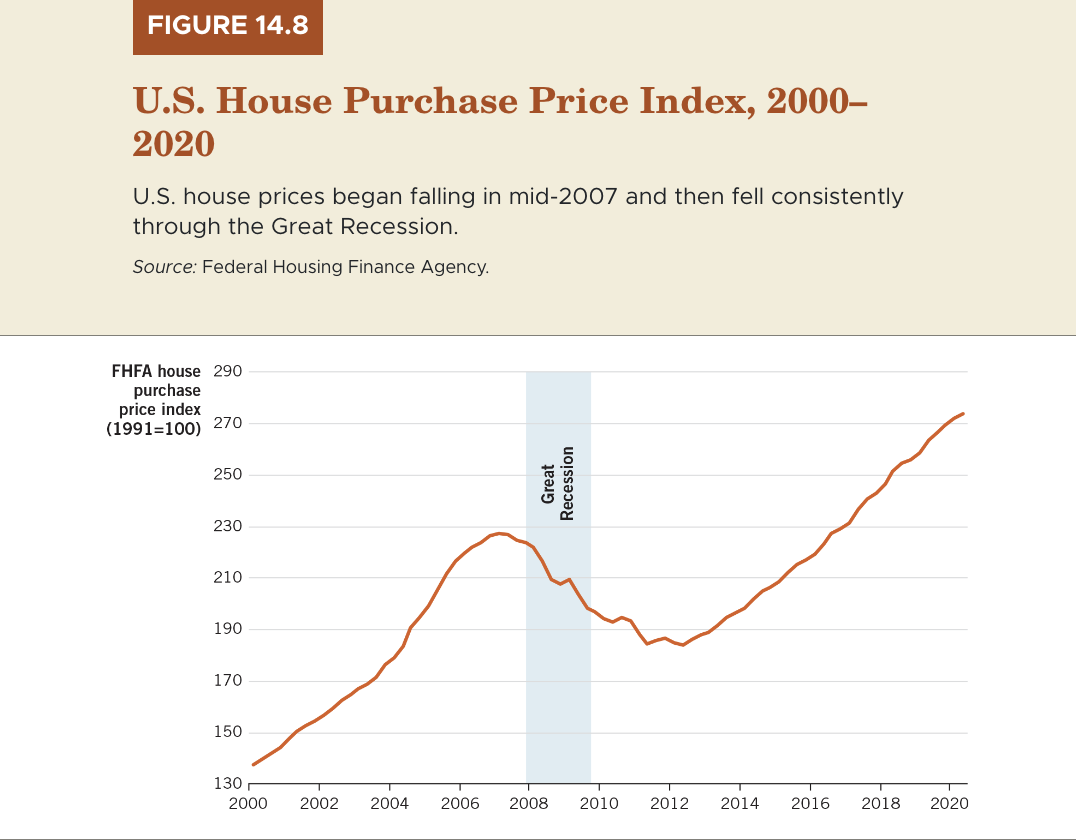
\includegraphics[scale=0.5]{images/Figure 14.8.png} 
\end{center}

Many economists feel that the troubles in hosing markets were related to U.S monetary policy - specifically, that there had been excessive monetary expansion in the previous decade. Looking again at Figure 14.8, you can see that housing prices rose significantly up to 2007 but then stalled. In \underline{Chapter 8}, we talked about the problem of price confusion: it arises when firms cannot tell whether price increases are due to real increases in demand or to inflation. This was the problem builders faced in the lead-up to the Great Recession; housing prices rose rapidly, but many economists now believe that this price "bubble" was a result of monetary expansion...in 2008, the bubble burst.

During this time, very large business firms, including financial institutions like Lehman Brothers, Bank of America, and Goldman Sachs, accumulated significant assets in the housing market, in particular in the market for securitized home mortgages. Recall from Chapter 10 that home mortgages were securitized into mortgage-backed securities and that significant quantities of these were held by most of the largest financial institutions. When real estate values fell, so did the values of those securities; now firms holding those securities had a cash flow problem on their hands. Because of the financial firms' interdependence, the problem quickly spread throughout the United States and then to the rest of the world; a financial crisis signals a breakdown in the loanable funds market. When the loanable funds market doesn't function properly, firms can't get funding to produce output, and aggregate supply falls.

Finally, new financial regulations enacted during the crisis changed the financial industry's operating environment. The \textbf{\underline{Dodd-Frank Act}}, signed in July 2010, was the primary regulatory response to the financial turmoil that contributed to the Great Recession. This act imposed new regulations in financial institutions and established several oversight bodies, with the goal of reducing risk in financial markets; but while the new regulations may have done that, they also affected banks' day-to-day operations. The new constraints represented a permanent change in how financial institutions operate and contribute to the reduction in long-run aggregate supply.

Consider an analogy in which financial markets are a bridge between savers and borrowers in an economy; funds flowing between between savers and borrowers are the "traffic" flowing across the bridge. If the economy is to grow, firms must be able to borrow, and so the bridge must be safe and efficient; financial crises are like accidents on the bridge that disrupt the flow of traffic and temporarily slow the economy. New financial regulations are like speed bumps or stricter speed limits, imposed to reduce the number of accidents and keep the traffic flowing; so while the new regulations can reduce instability in financial markets, we also acknowledge that fewer risky loans might also reduce growth in expansionary periods. In our model, we illustrate the permanent effects of the financial crisis and changes in institutions as a decline in long-run aggregate supply.

Figure 14.9 shows a decline in both aggregate demand and aggregate supply from 2007 to 2008. Aggregate demand shifted from \(\text{AD}_{2007}\) to \(\text{AD}_{2008}\), and long-run aggregate supply shifted from \(\text{LRAS}_{2007}\) to \(\text{LRAS}_{2008}\). (Short-run aggregate supply is not pictured here; it shifts with the long-run aggregate.) In 2007, the economy was in equilibrium at point A; at this time, the unemployment rate (not pictured in Figure 14.9) was below 5\%, and real GDP (\(Y\)*) was growing at a 3.6\% rate in the second quarter of 2007.

Then conditions worsened as housing prices fell and financial market turmoil ensued, leading to lower real wealth and then to lower consumer confidence. The declines in aggregate demand and long-run aggregate supply moved the economy to a new equilibrium at point B. During this time, the unemployment rate climbed to 10\%, and by the last quarter of 2008, real GDP was declining by 8.9\% (on an annual basis). The unemployment rate rose significantly beginning in 2008 and then continued for several years. This was due in part to an increase in cyclical unemployment, but it was due in part to an increase in structural unemployment as the economy adjusted to new types of output in the wake of a decline in long-run aggregate supply.

\begin{center}
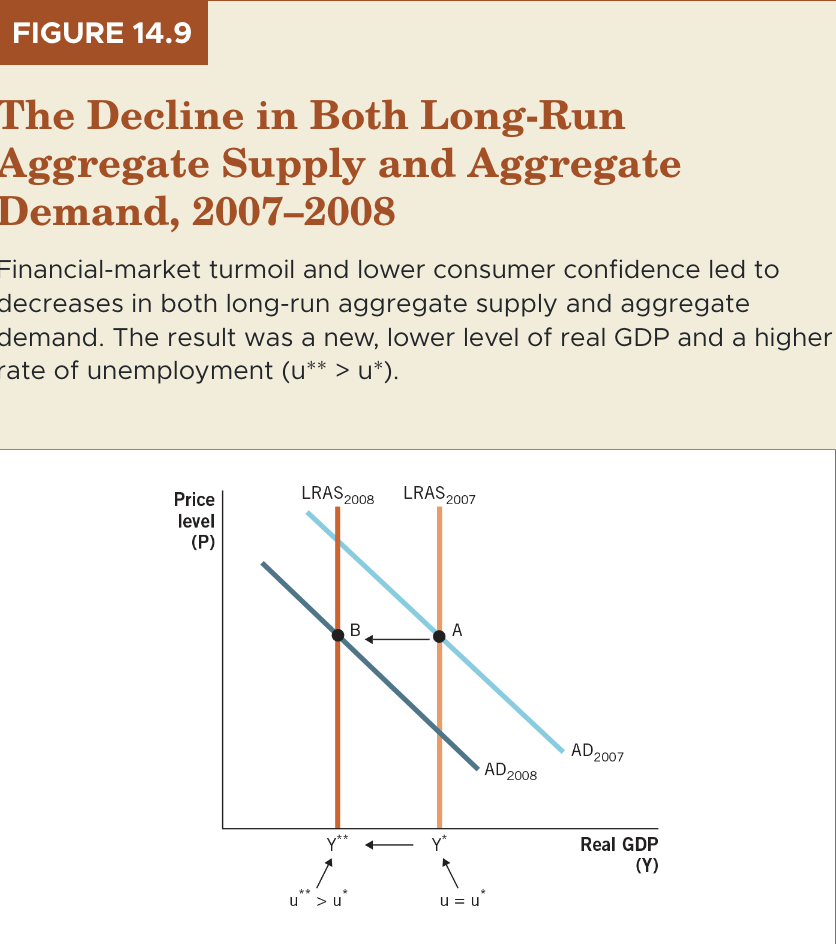
\includegraphics[scale=0.5]{images/Figure 14.9.png} 
\end{center}

\subsection*{The Coronavirus Recession}
In early 2020, the U.S economy was experiencing it's longest expansion on record: real GDP had grown for more than a decade, and the unemployment rate was just 3.5\%, its lowest level since 1969. In the language of macroeconomics, the U.S economy was at or near its full-employment level; elsewhere, conditions were similarly favorable: the unemployment rate was 7.3\% in Europe, 4.4\% in China, and just 2.5\% in Japan.

However, a worldwide catastrophe was unfolding; on January 1, 2020, Chinese government health inspectors at a market in Wuhan city took germ samples and cleansed parts of the market, hoping to contain an outbreak of a new type of coronavirus. Unfortunately, their efforts fell short; by January 23, when Wuhan's 11 million residents went into lockdown, the virus had already escaped and begun its spread across the globe.

The first coronavirus infection in the United States was diagnosed on January 20, 2020; the economy went into recession seven weeks later, right around March 10, as people began social distancing , travel was widely banned, and many U.S states started restricting large gatherings. Major League Baseball and the NBA postponed their seasons; college athletic events, including the March Madness basketball tournament, were canceled; Restaurants, movie theaters, airports, and retail stores closed their doors; universities sent students home and shifted to online instruction. We can't usually pinpoint the exact beginning of a recession, but here we can; you likely recall this period vividly, as daily life instantly changed for almost everyone.

\subsubsection*{The Magnitude of the Coronavirus Recession}
Figure 14.10 shows U.S real GDP and the unemployment rate from the year 2000 to end of 2021. In both panels, the COVID-19 recession stands out dramatically; looking at panel (a), you can see the "cliff" in the second quarter of 2020, where the U.S economy plunged into recession, real GDP fell 9\% in that quarter alone. This translates to a 31.7\% annual drop - the hypothetical rate of decrease if the quarterly drop lasted a whole year; panel (b) shows the effect of on the unemployment rate. In April of 2020, the rate climbed to 14.7\%, its highest point since the Great Depression.

However, the COVID-19 recession stands out in the data not only because it came on so quickly but also because of the rapid recovery. By early 2021, real GDP was back to its pre-recession level, and by the end of 2021, the unemployment rate had dropped back below 4\%.

\subsubsection*{Using our model to explain the coronavirus recession}
The coronavirus recession was different from the other two recessions we consider in this chapter. Most importantly, the main driver of this downturn was a global pandemic; remember our definition of a supply shock: a surprise (exogenous) event that changes production costs. A pandemic is a classic short-run supply shock that shifts the short-run aggregate supply curve to the left. The COVID-19 pandemic was far worse than other recent pandemics (like SARS in 2003 and the H1N1 swine flu in 2009), but it affected the economy in the same basic way - just much more severely. While the primary and largest cause of the 2020 recession was on the supply side, aggregate demand also fell; real wealth fell, and extreme uncertainty reduced expected future income, both of which led to a decrease in AD.

\begin{center}
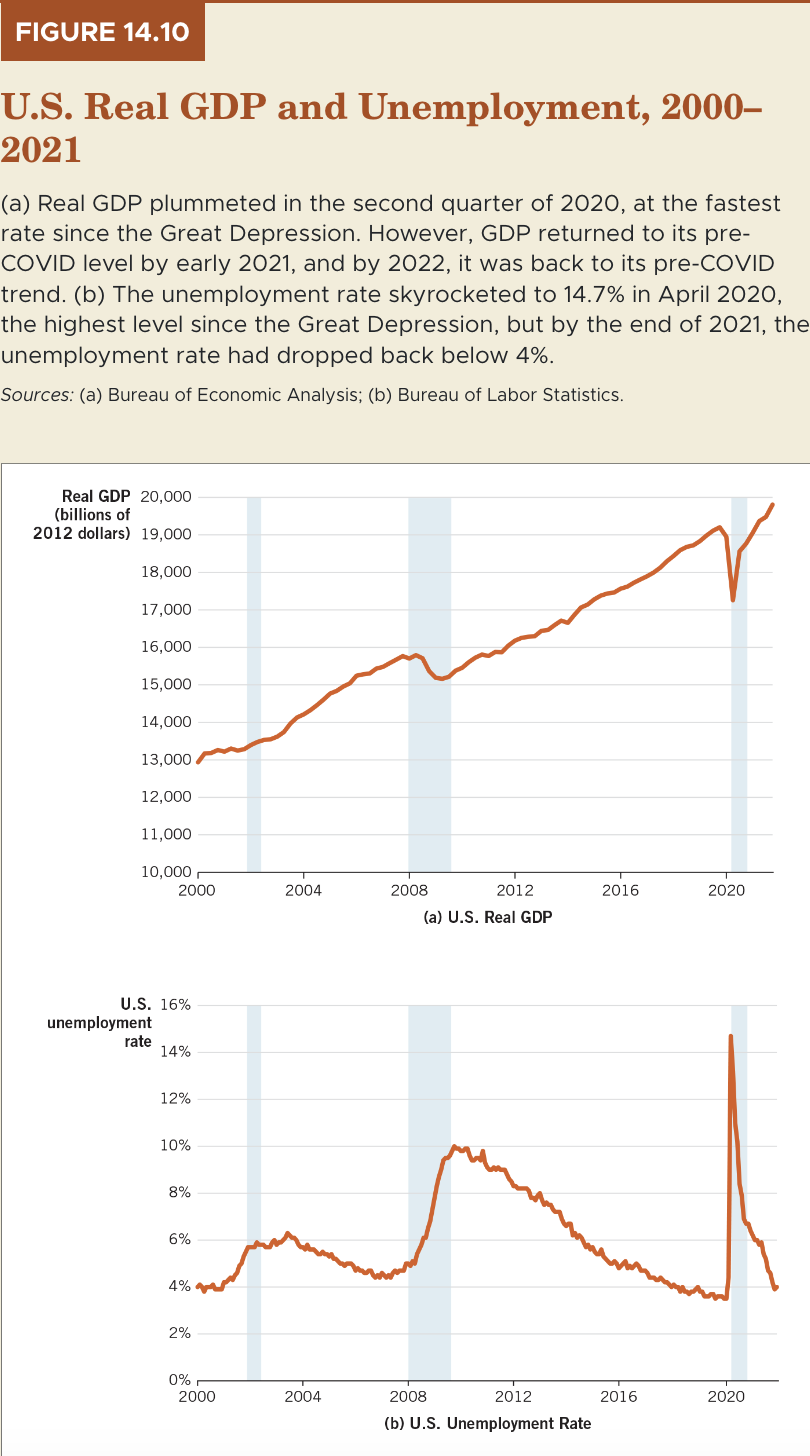
\includegraphics[scale=0.5]{images/Figure 14.10.png}
\end{center}
Figure 14.11 illustrates these changes in the U.S economy; at the end of 2019, the economy was in long-run equilibrium at point A, with short-run aggregate supply \(\text{SRAS}_{2019}\), long-run aggregate supply LRAS, and aggregate demand \(\text{AD}_{2019}\). The unemployment rate was below 4\%, and real GDP increased by 2\% in 2019

By the following March, however, much of the U.S economy was shutting down. You can see this in the model: short-run aggregate supply declined to \(\text{SRAS}_{2020}\), and aggregate demand decreased to \(\text{AD}_{2020}\). The reduction in SRAS followed increased production costs, due to factors like social distancing, international shipping interruptions, and general health risks form the virus itself. Think of what restaurants in your area had to do to stay open; many found a way to provide outdoor seating, but the tents and awnings cost money, and so did the extra time it took the servers to bring food out to the tables. Even then, restaurants couldn't accommodate as many patrons as before, and they had difficulty hiring workers who were fearful of being exposed to the virus. That is what aggregate supply shifting left looked like: a lot of firms had to spend more to produce less.

\begin{center}
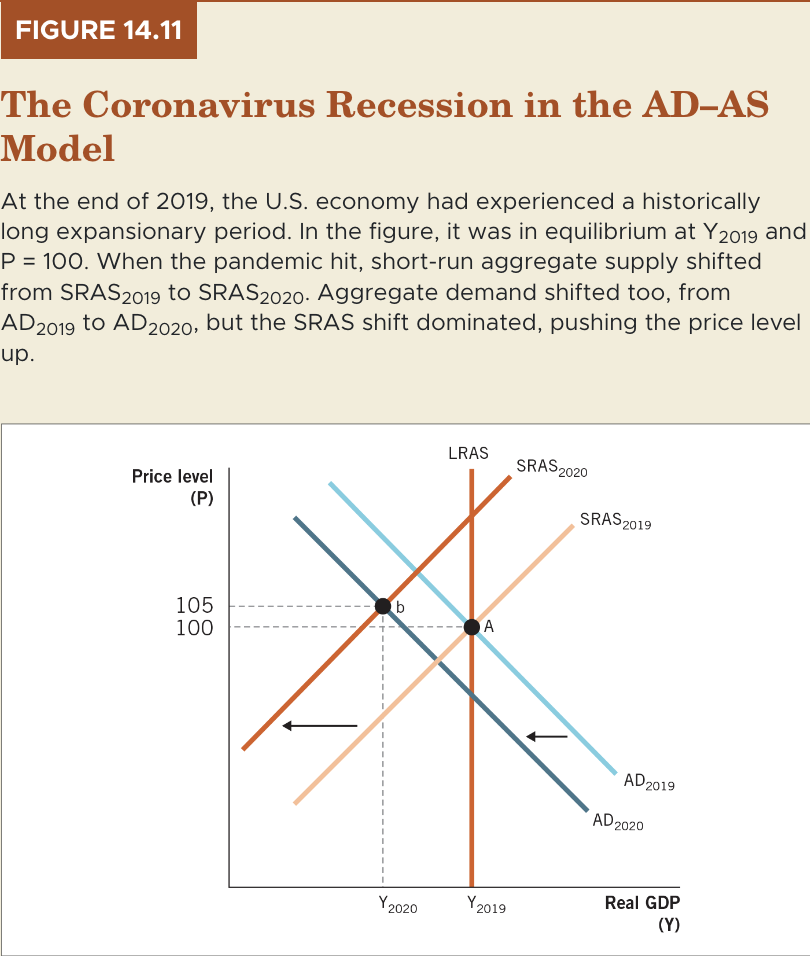
\includegraphics[scale=0.5]{images/Figure 14.11.png}
\end{center}
After the shifts in SRAS and AD, the new short-run equilibrium was at point b with higher prices, lower real GDP, and higher unemployment. In the long run, as infection rates fell and behavior returned to normal (or close to it), SRAS and AD shifted back to the right, and the economy returned to long-run equilibrium. You can see this in Figure 14.10; the big plunge is the original leftward shift in SRAS, and then, quarter after quarter, the economy moves back toward its pre-COVID state.

\section*{What are the big disagreements in macroeconomics?}
We now consider the major debates in macroeconomics by building on our discussion of the Great Depression; most economists agree with the basic implications of the aggregate demand-aggregate supply model. However, economists disagree about the role of government and the economy's ability to self-correct; in this section, we try to clarify some of the issues on which this debate turns.

Perhaps the most contentious issue among macroeconomists involves the economy's adjustment to long-run equilibrium; consider again the short-run equilibrium, $b$, in Figure 14.1. Some economists believe that adjustment can and should occur naturally; this group, broadly called \textbf{classical economists}, emphasize that all prices eventually adjust and that the economy goes back to long-run equilibrium, at point C. Others, called \textbf{Keynesian economists}, see the return to long-run equilibrium as a delayed, unpredictable adjustment; this group stresses the importance of aggregate demand and calls for the government to speed up the process back to full employment by shifting the aggregate demand using fiscal and monetary policy. While not every economist fits completely in either camp, these distinctions help clarify the debate.

\subsection*{Classical Economics}
At the beginning of the twentieth century, economic theory was basically what we now think of as microeconomics. Economists had a good sense of the merits of supply and demand analysis for individual markets; as you know, when we consider basic supply and demand, the price of the good adjusts to draw the market toward equilibrium. To the extent these economists considered macroeconomic issues, they extended their ideas from microeconomic analysis; in particular, their faith in price flexibility extended to their view of the macroeconomy.

Thus, flexible prices form the foundation of the classical view of the macroeconomy; consider the implications: if prices are completely flexible, the economy is essentially self-correcting. No matter what factors change in the economy, no matter which curves shift, with fully flexible prices the economy automatically maintains full employment (illustrated by the vertical long-run aggregate supply curve).

\begin{center}
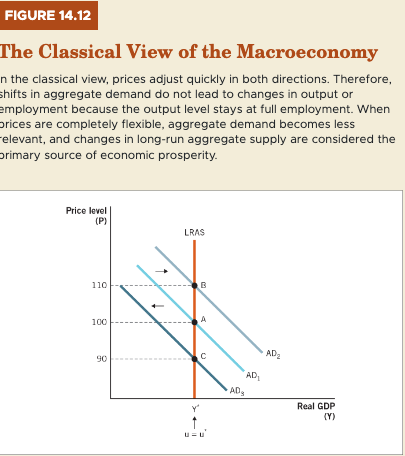
\includegraphics[scale=0.5]{images/Figure 14.12.png} 
\end{center}
If prices are completely flexible, the economy quickly settles back at full-employment output and the natural rate of unemployment; classical economists probably sleep well at night; without worries about long-term economic contractions.

Because they believed that economy self-corrects back to full employment, classical economists were essentially laissez-faire in their policy recommendations. They had faith that market adjustments would take place quickly, so they saw no significant role for a government macroeconomic policy focusing on short-run fixes when the economy is underperforming or overperforming.

\subsection*{Keynesian Economics}
Although the classical economists dominated economics early in the twentieth century, the experience of the Great Depression presented the challenge to the accepted wisdom. The Great Depression set the stage for a new approach to macroeconomics; John Maynard Keynes, a British economist, formulated this new doctrine. In 1936, Keynes published \textit{The General Theory of Employment, Interest, and Money}; this book vaulted him into the forefront of macroeconomic debates because it offered a theory about why recessions might last a while, indeed, the title of the book - \textit{The General Theory} - implies that Keynes believed that an economy out of long-run equilibrium is not unusual. Proponents of this view became to be know as Keynesian economists.

Keynesian economists emphasize that after a decline in aggregate demand, some prices, particularly wages, are very slow to adjust downward to move the economy back to full employment. In short, wages and certain other prices are "sticky"; as a result, high real wages prevent the labor market from reaching equilibrium and restoring full employment. Here we have an explanation for how prolonged recessions can happen; Keynes advocated governmental intervention to move the economy back to full employment. He argued that the government should try to shift the aggregated demand curve back to its initial level; according to Keynes, it is foolish to wait for long-run adjustments because, as he famously said, "In the long run we are all dead".

To the extent that wages and other prices are indeed sticky, demand declines spell serious trouble for the economy, because there is no natural adjustment back to full employment. So Keynesian economists focus on the demand side of the economy as the source of instability.

Why would wages and other prices be sticky? One explanation is the presence of long-term wage contracts, especially when negotiated through collective bargaining agreements by unions. Certainly, a larger percentage of the labor force was unionized in the 1930's, and this no doubt contributed to wage rigidity; but money illusion may also played a role (see \underline{Chapter 8}). Imagine yourself as an employee in the midst of the Great Depression: times are tough, and now your employers is asking you to accept lower wages...this is a tough pill to swallow, even if, with falling consumer prices, you're not looking at a 
\text{real} wage decrease. You, or some of your coworkers, might refuse a wage cut; employees who refuse a paycut might lose their jobs; this begins a troubling cycle, as workers, as without jobs drastically cut their spending, and this leads to a reduction in economic activity. Recall the circular flow diagram  as we discussed Chapter 7; the welfare of businesses and workers interwined.

Keynes recommended that the British and U.S governments take action to increase aggregate demand. Keynes felt that, with additional government spending, governments could play a role in stopping the global economy's decline; government spending can increase aggregate demand. Keynes recommended fiscal policy in the form of spending on social programs and additional infrastructure (we discuss this further in Chapter 16); during the Great Depression, a host of programs put into place as part of Franklin Delano Roosevelt's New Deal were designed to create immediate jobs and spending in the economy. If aggregate demand is too low because individuals and firms are reluctant to spend, Keynes argued, the government might fill the void by increasing the government-spending piece pf aggregate demand.

The Keynesian view of the economy offered an explanation for the Great Depression; in fact, after the nation emerged from the Great Depression, Keynesian theory became dominant in the field of economics.

\textbf{Table 14.1 summarizes the major differences between classical and Keynesian economists.}

\begin{center}
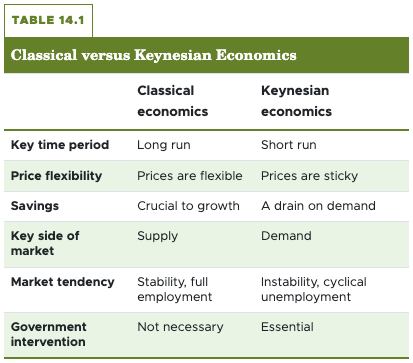
\includegraphics[scale=0.5]{images/Table 14.1.png} 
\end{center}

\section*{Conclusion}
We began this chapter with a look at the severity of the Great Depression; while every recession brings hardship, we have seen that no other modern recession was nearly so severe as the Great Depression. We've now also considered two different views of the macroeconomy: the classical view and the Keynesian view; the views of the most economists probably fall on a continuum between these two views, some emphasizing price adjustments and the importance of supply and others emphasizing price stickiness and the importance of demand. But most also see a role for governmental policy, especially during downturns when resources are idle.

Going forward, we can use the aggregate demand-aggregate supply model as a tool for analyzing government policy. This include monetary policy, which adjusts the money supply, and fiscal policy, which adjusts taxes and spending; over the next four chapters, we evaluate these policy alternatives and use the aggregate demand-aggregate supply model to understand how governmental policy affects the economy. 

\end{document}
